\ejercicio{Recorrer el arreglo con bucle for}

Con un bucle for, recorrer el arreglo y mostrar todos los datos de los objetos por pantalla.

\codigojava{ejercicios/ej04/Ejercicio04.java}

\newpage
\vspace{1em}
\textbf{Salida del programa:}
\vspace{0.5em}
\begin{figure}[H]
    \centering
    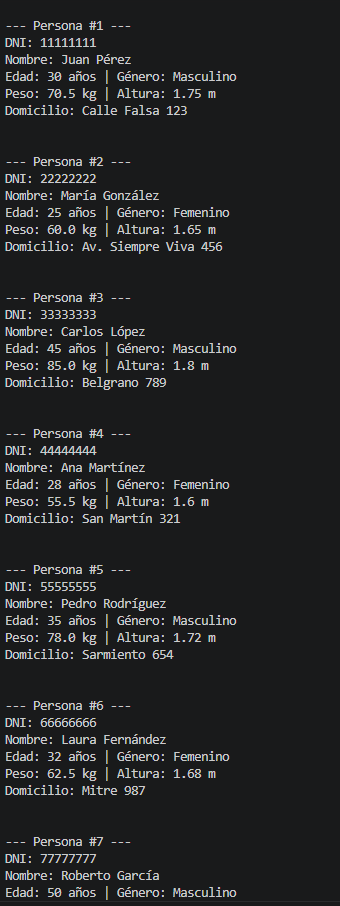
\includegraphics[width=0.5\textwidth]{ejercicios/ej04/captura1.png}
\end{figure}
\vspace{1em}

\vspace{0.5em}
\begin{figure}[H]
    \centering
    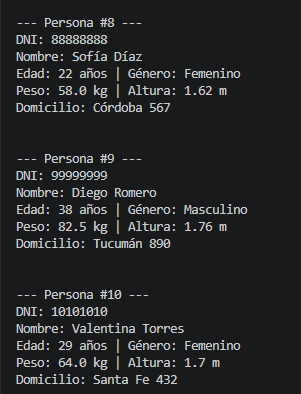
\includegraphics[width=0.5\textwidth]{ejercicios/ej04/captura2.png}
\end{figure}

\volverindice
\newpage